\chapter{Results}
\label{results}

\minitoc

In this chapter results from the case study will be highlighted. Starting of the chapter is an introduction and overview of the Omega-project, as well as a classification of the project in a multi-team system context. When this is performed the findings from all three focus groups are presented.


\newpage

\section{Clarification}

Before giving an overview of the Omega-project, both in a general fashion and in a multi-team system context, it is important to clarify that all quotations used in this chapter are translated from Norwegian to English by the researcher. The reason for this is because the focus groups and interviews carried out in the case study were conducted in Norwegian.

\section{Overview of the Omega-project}

To start of the result chapter it is important to get a clear overview of how the project was organised and conducted. The Omega-project was initiated and conducted by the public sector department Gamma. Gamma saw a need for a new office automation system, and especially argued that a new system was needed because the current platform was outdated and about to be abandoned. It is important to note that with the commencement of the Omega-project little was known about the content of the public reform, and therefore an agile development methodology and mindset was selected to take into account the high level of uncertainties and complex nature of the proposed project.

Omega is one of the largest IT development projects in Norway to date, consisting of approximately 175 members, where 100 of these came from five external companies. The project had a final budget of roughly 140 million euro. It lasted for about four years (January 2008 to March 2012) and had a strict deadline because of the reform. Around 800.000 person hours were used in developing {\raise.17ex\hbox{$\scriptstyle\mathtt{\sim}$}}300 epics with a total of {\raise.17ex\hbox{$\scriptstyle\mathtt{\sim}$}}2500 user stories. All of these were divided into 12 main releases (there were also smaller releases throughout the project). Figure \ref{releases} shows how these 12 releases where located in the timeline of the project.

\begin{figure}
\centering
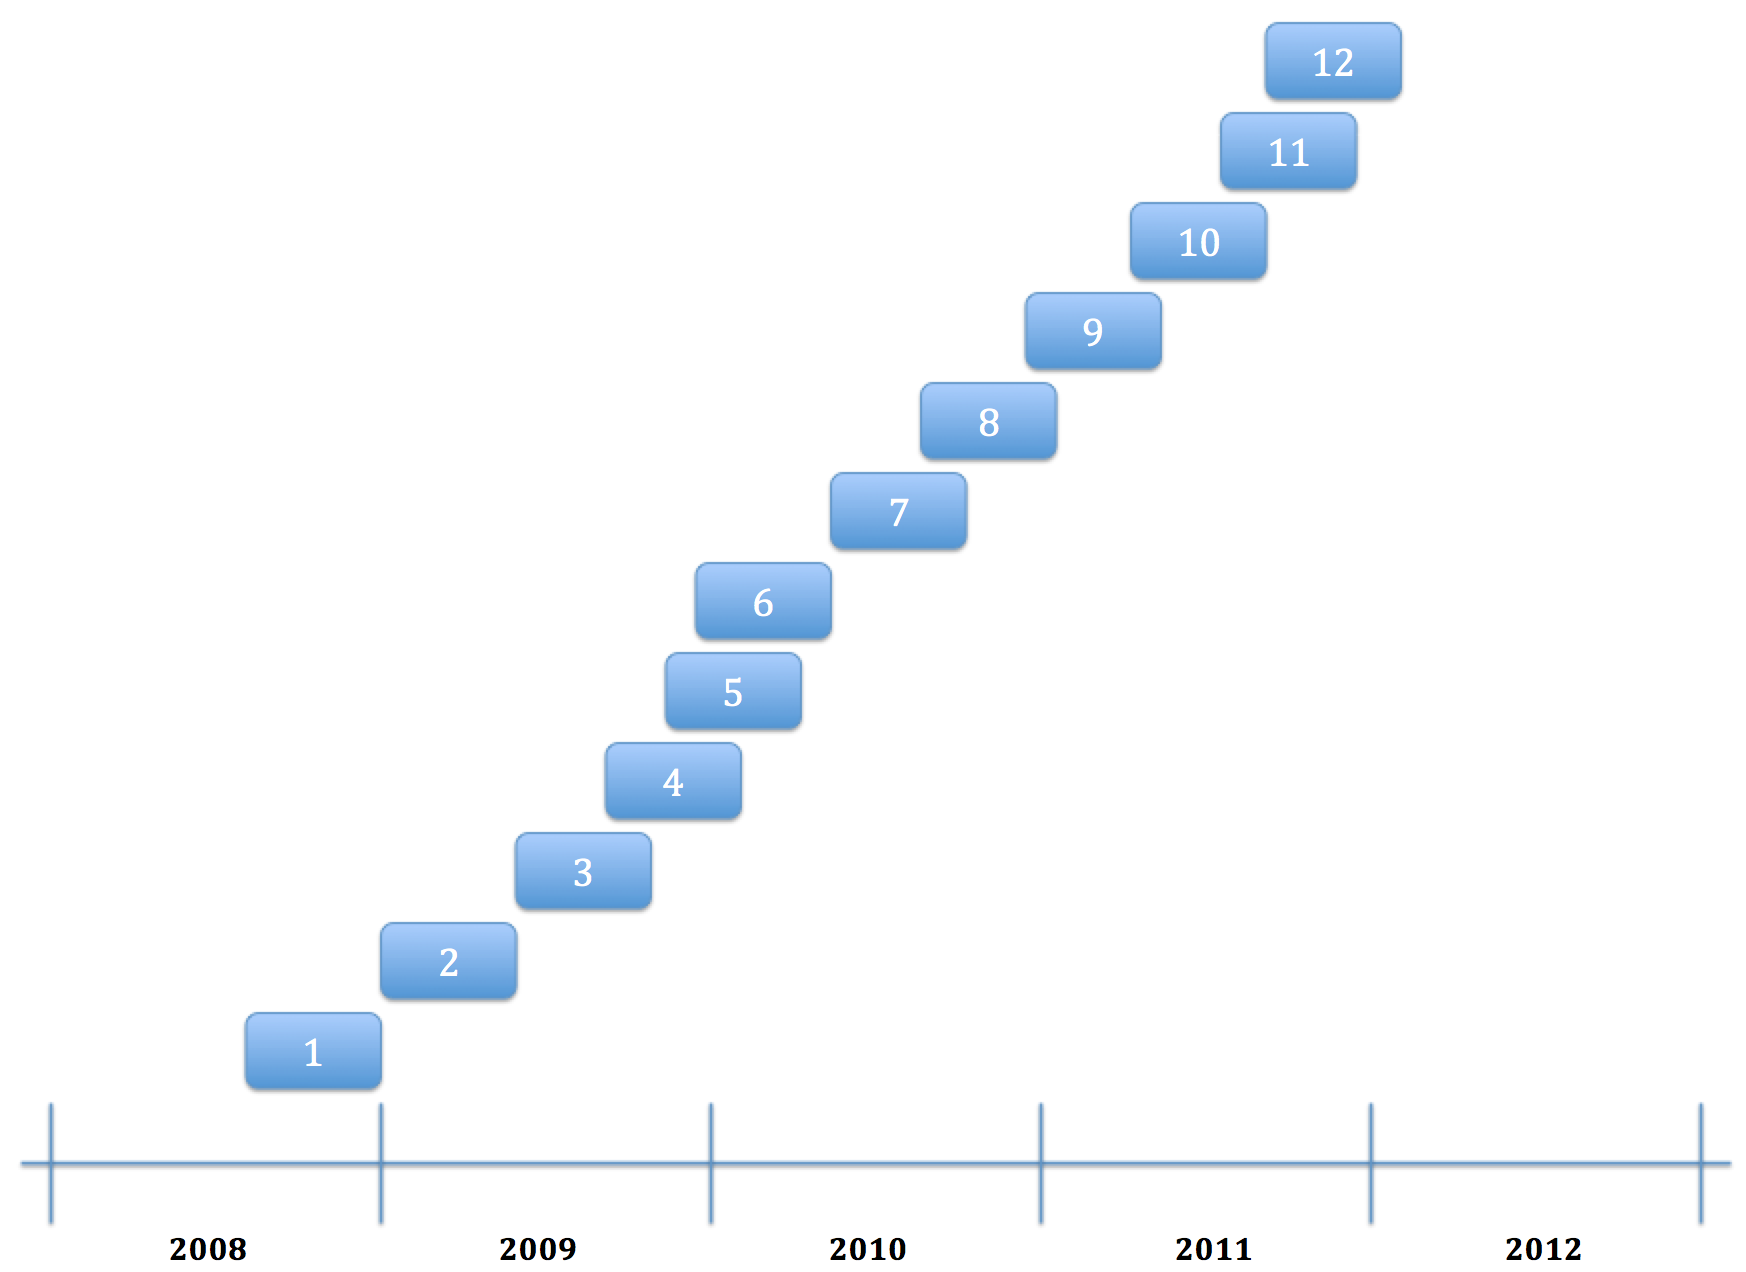
\includegraphics[trim = 0mm 0mm 0mm 0mm,width=155mm]{images/project_releases}
\caption{Main project releases in Omega.}
\label{releases}
\end{figure}

The initial project execution model consisted of six phases involving different personnel. The planned project execution was as follow: Starting of the project was a general requirements phase where potential impacts also were assessed. Here both business resources and architects were present. Following the general overview phase was a requirements analysis phase, again with both business and architecture resources. After these more general phases the solution description was worked on. The solution description was the main responsibility of the architecture unit, but business resources, developers, test resources and the heads of delivery were included. Going into the construction and approval phases all resources were collaborating to get continuous deliveries finished for production. In the production phase the main responsibility was put on the heads of delivery, but business and line resources were also present throughout the whole process, and architects, developers and testers were included in parts of the phase. The whole project execution model can be seen in figure \ref{project_execution}.

\begin{figure}
\centering
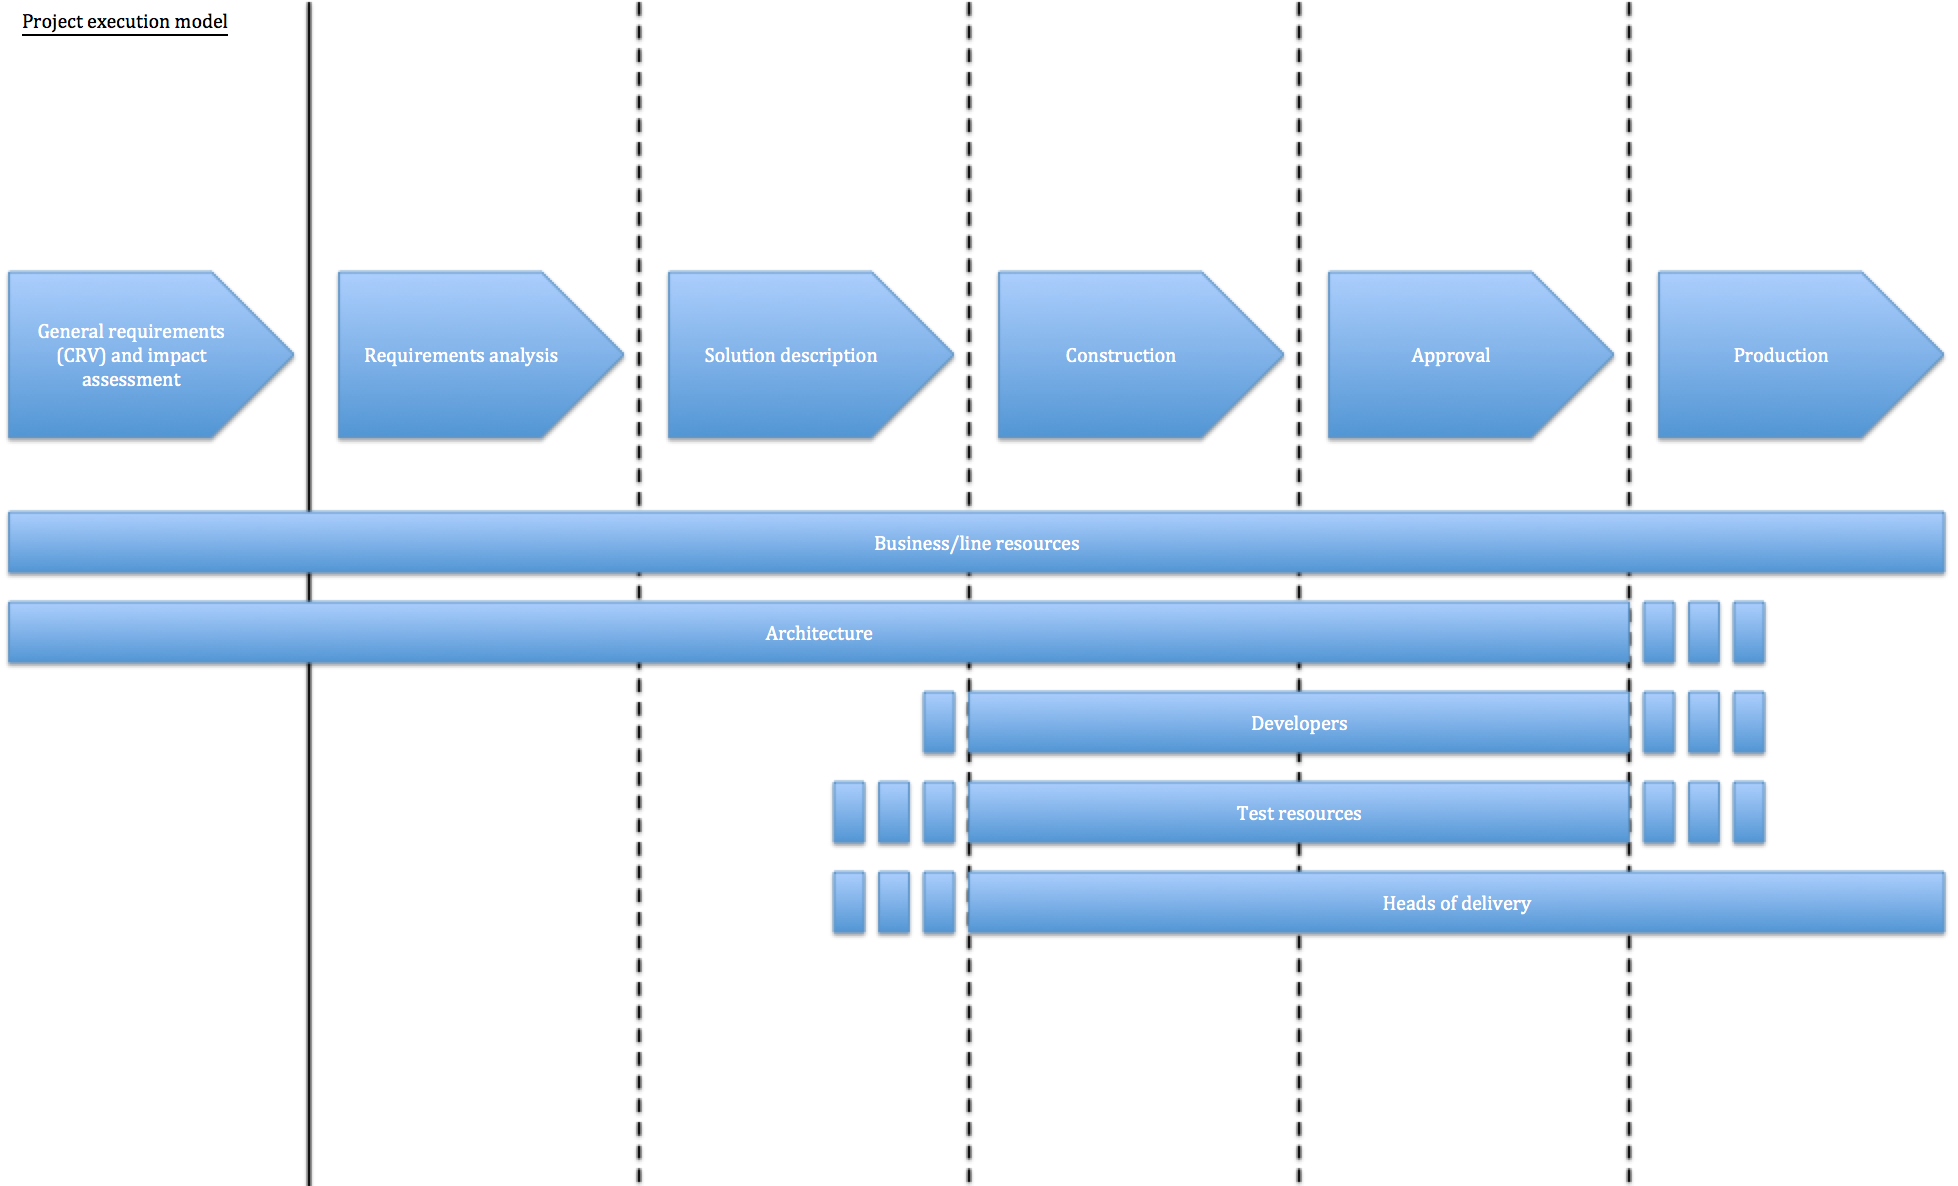
\includegraphics[trim = 0mm 0mm 0mm 0mm,width=155mm]{images/execution_model.png}
\caption{Project execution model.}
\label{project_execution}
\end{figure}

The project was organised with a ``project director'' at the top of the hierarchy mainly focusing on external relations. Underneath the project director there was a ``project manager'' responsible for operations. Omega also had four sub-projects with one ``sub-project manager'' each. These sub-projects were architecture, business, development and test, and are further described below. There were also a ``controller'' (or ``secretary'') present for administrative reasons. As can be seen from figure \ref{omega} the project used a matrix structure where the business and development sub-projects were both closely linked to the test and architecture sub-projects.

%TODO: Endre Alfa til Alpha
\begin{figure}
\centering
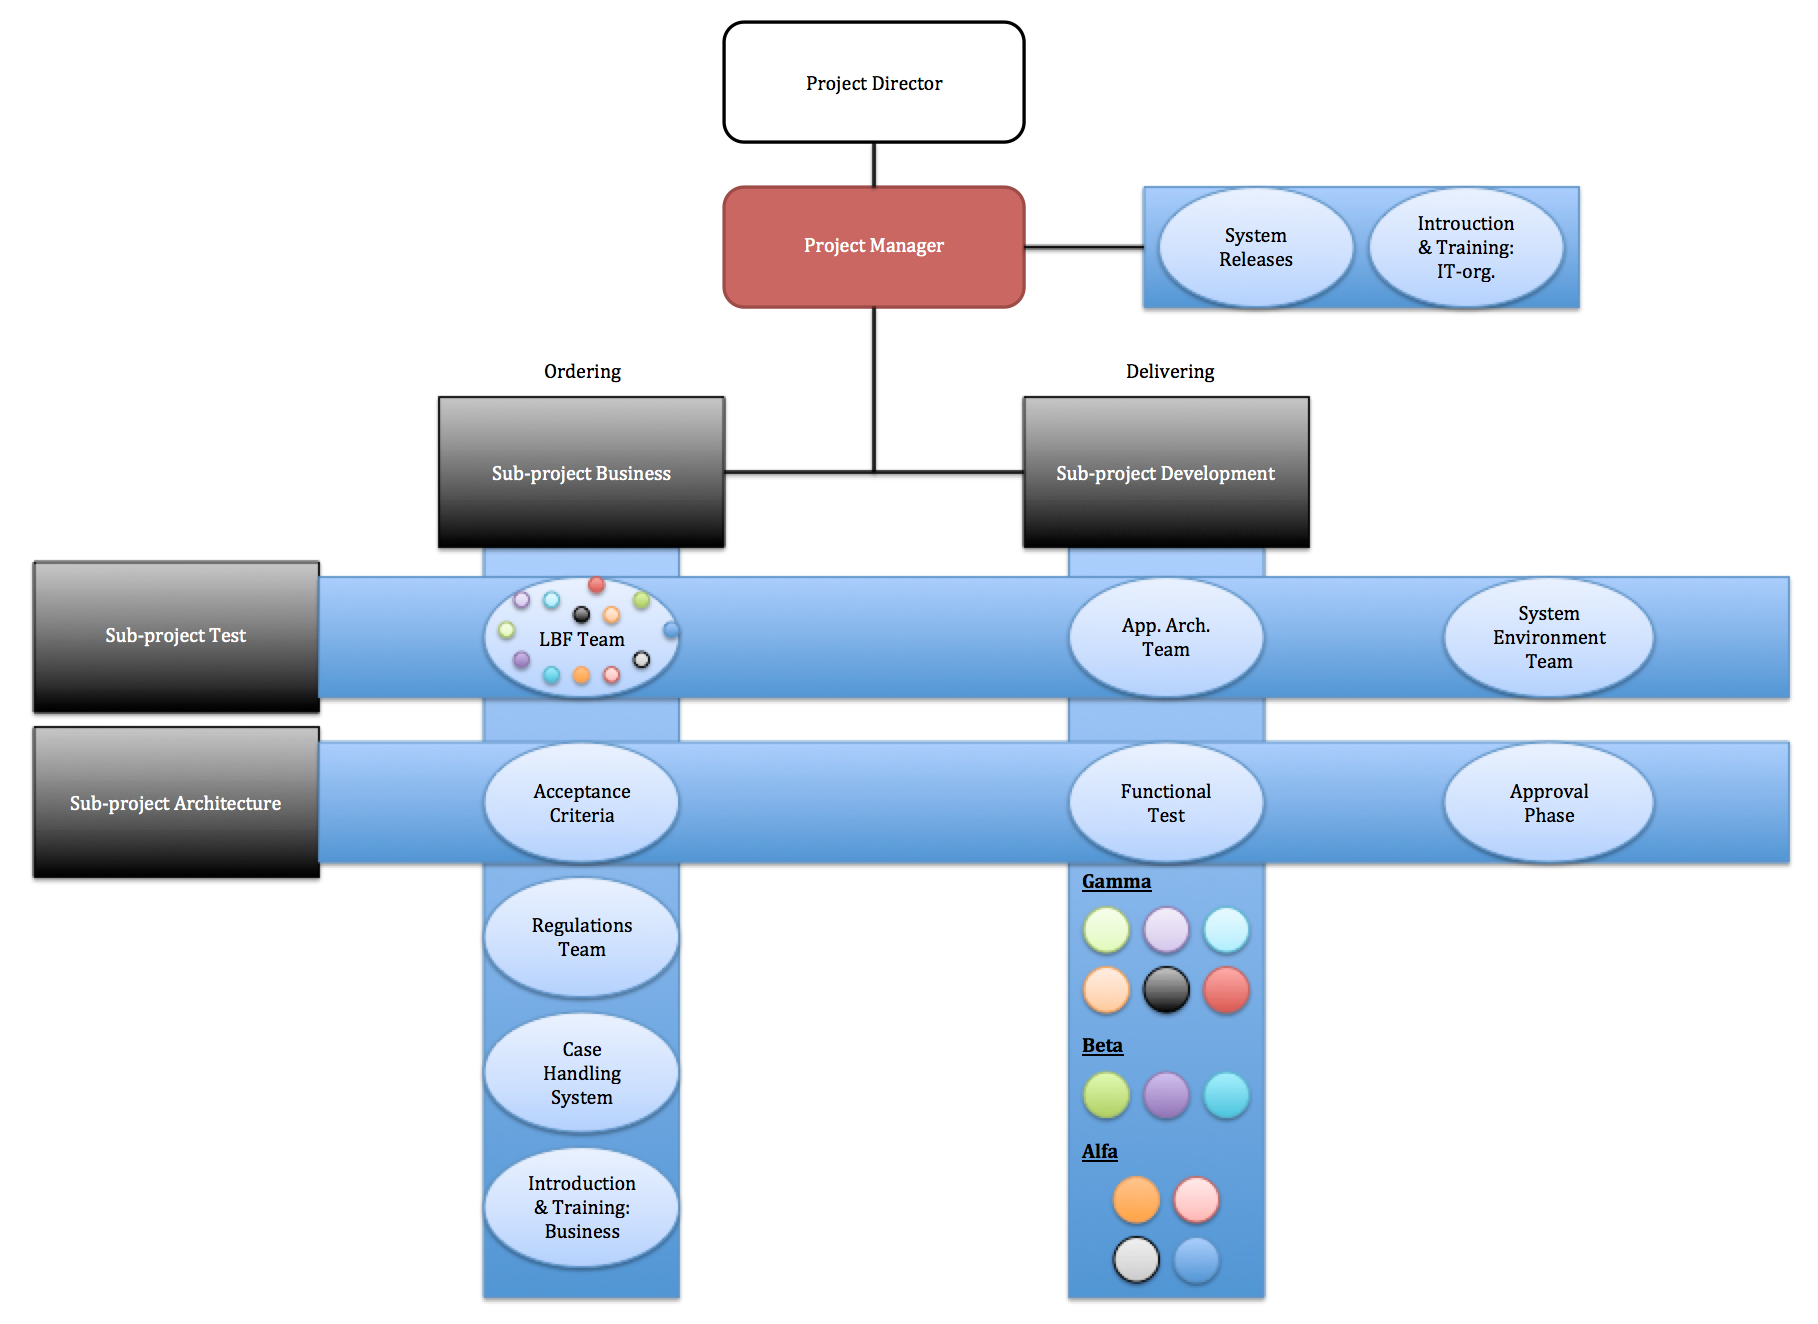
\includegraphics[trim = 0mm 0mm 0mm 0mm,width=155mm]{images/omega_organisation.png}
\caption{Omega-project's organisation.}
\label{omega}
\end{figure}

\begin{itemize}
   \item \textbf{Architecture:} Architects were in general responsible for the overall architecture of the project, but more specifically focused on solution description. They were also important in dealing with dependencies in Omega, and continuously updated a dependency map. The sub-project had head architects at a project management level and technical and functional architects located on a team level.
   \item \textbf{Business:} The business and line resources were present in the whole execution of the project (as can be seen from figure \ref{project_execution}). The responsibility of the business sub-project was to categorise needs and requirements, and then defining these into epics and user stories in a product backlog. In this sub-project there was a product owner team, but also other business and line resources (approximately 30 members at a peak period). Both functional and technical architects from the Scrum teams were also involved in the business sub-project.
   \item \textbf{Development:} The construction sub-project was further divided into three sub-projects led by Alpha, Beta and Gamma. The Gamma organisation had at most six development teams involved with both their own personnel and external consultants hired in from five different consulting companies. Alpha had at most four teams, while Beta had a maximum of three development teams. All 13 component teams worked corresponding to the Scrum methodology and delivered on a common demo day at the end of every three-week sprint iteration. There was also a system environment team present which was in charge of development and test environments. All roles of the Scrum teams are outlined in table \ref{trpist}.
   \item \textbf{Test:} The test sub-project had responsibility for all the testing of the project and the providing of deliverables from the development teams. Hence, they were important for quality assurance. The sub-project included a test leader, as well as test personnel from the development teams.
\end{itemize}

The main focus of this master thesis has been on the development of the system, and the personnel involved in this process. The development iterations had four phases: ``analysis of need'', ``solution description'', ``construction'' and ``approval''. These are further described below. The development process can be seen in figure \ref{initial_development_process}.

\begin{itemize}
   \item \textbf{Analysis of need:} Starting of each development release was an analysis phase. Here the focus was on functionality to be included in the coming release, and identifying and working out user stories. The product owner was involved in this process and was, e.g., responsible for prioritising the product backlog.
   \item \textbf{Solution description:} After identifying and working out general user stories in the ``analysis of need'' phase the user stories were further developed and made more comprehensive in the ``solution description'' phase. These user stories were also assigned to epics, and further estimated in approximate work-hours to completion before being assigned to different Scrum teams. Design and architectural choices were also determined in this phase.
   \item \textbf{Construction:} The construction phase typically consisted of five to seven sprint iterations per main development release. Here all development was carried out, and all work was functionally tested.
   \item \textbf{Approval:} In the last phase of each development release the delivered functionality was tested, both formal and non-formal functional testing was performed. This was done to assure both the internal and external interfaces were working as expected.
\end{itemize}

\begin{figure}[H]
\centering
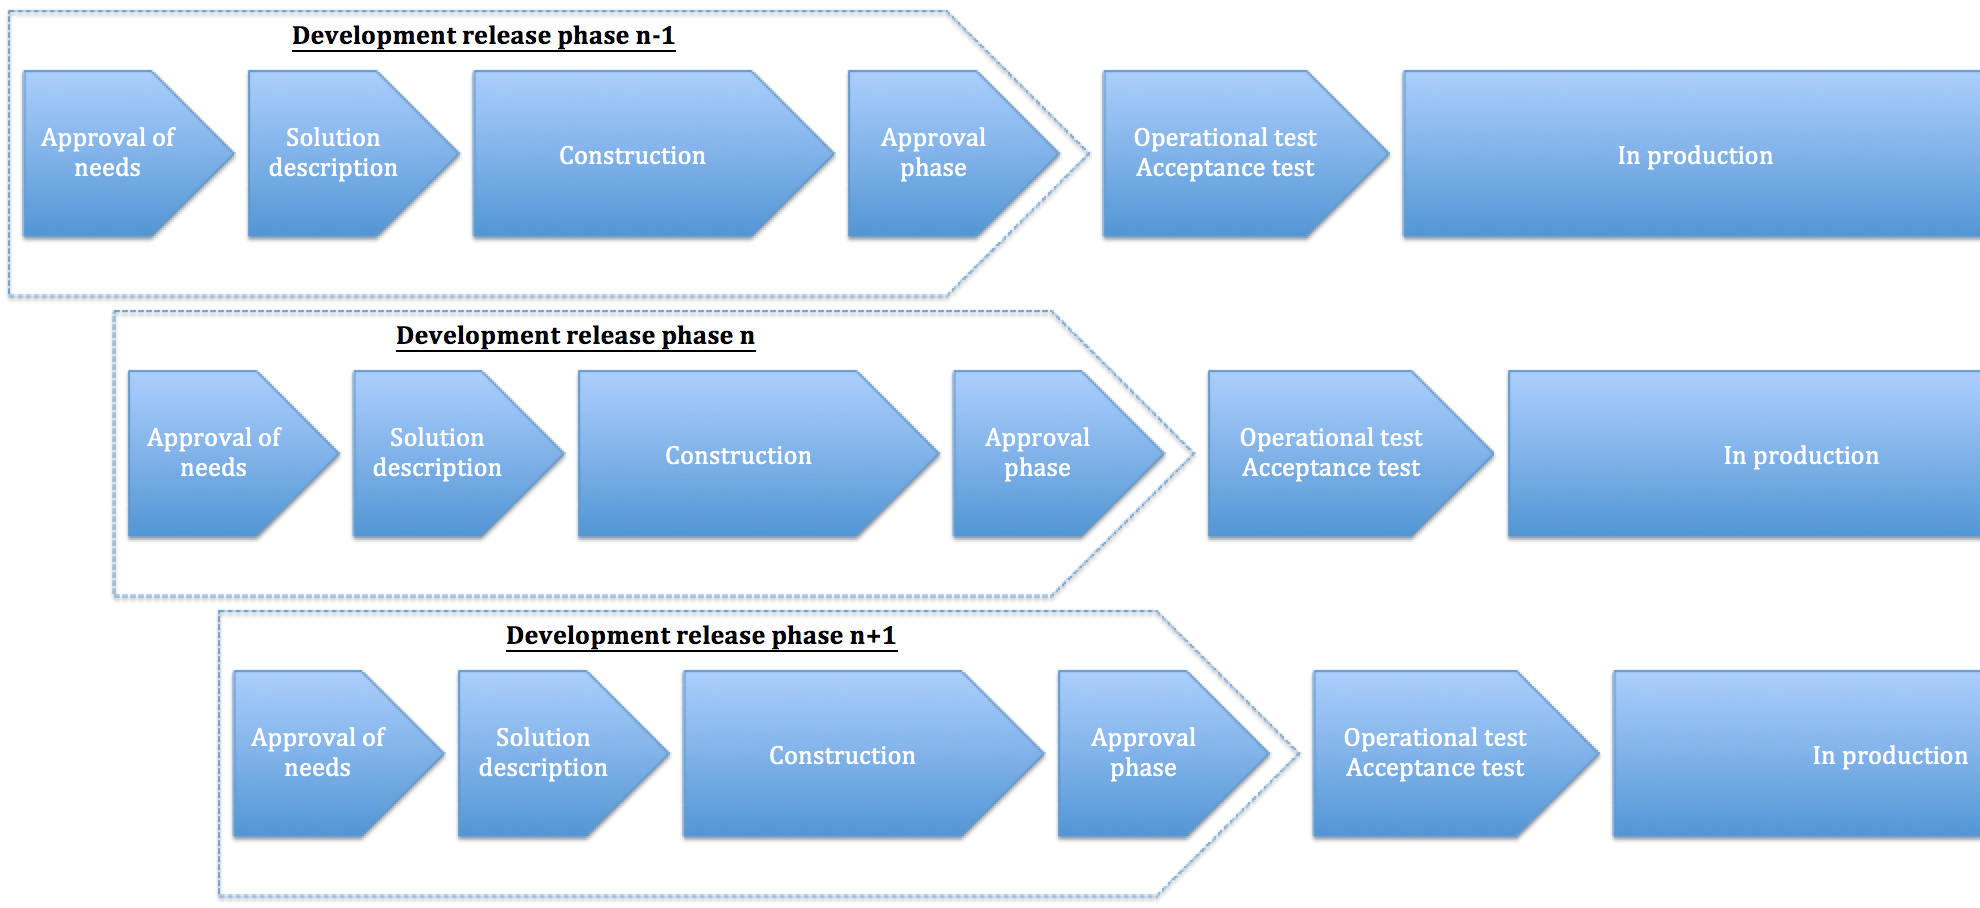
\includegraphics[trim = 0mm 0mm 0mm 0mm,width=155mm]{images/initial_development_process}
\caption{Initial development process.}
\label{initial_development_process}
\end{figure}

The development phase consisted primarily of several Scrum teams typically involving eight to nine members each. The roles in the different Scrum teams are further outlined in table \ref{trpist}. It is however important to remember that all members were somewhat cross-functional in the project. This means that a tester could for example have been 60\% tester, 30\% developer and 10\% designer, and a Scrum master could have been 50\% leader, 30\% architect and 20\% developer. 

\begin{center}
    \begin{longtable}{| p{4cm} | p{8cm} |}
   
    \hline \textbf{Role} & \textbf{Description of role} \\ \hline
    \endfirsthead

    \multicolumn{2}{c}%
{{\bfseries \tablename\ \thetable{} -- continued from previous page}} \\ \hline
    \textbf{Role} & \textbf{Description of role} \\ \hline
    \endhead

    \multicolumn{2}{|r|}{{Continued on the next page\ldots}} \\ \hline
    \endfoot

   \endlastfoot 

    Scrum master & The Scrum master facilitated all meetings such as the daily stand-up, demo presentations, retrospectives and iteration planning. Some teams rotated the role, while others had a fixed Scrum master. \\ \hline
    Functional architect & The functional architect was typically working 50\% with analysis and design, and 50\% as a developer. \\ \hline
    Technical architect & About half of the time went towards technical design, while the other half usually was spent developing. \\ \hline
    Tester & The person with the title ``tester'' was not responsible for doing all the testing, but was rather responsible for the tests being conducted. He was also in charge of writing and delivering test criteria to the sub-project test. The tests at the team level was unit tests, integration tests, system tests and system integration tests. Some of the teams did not have fixed testers, but rotated the role somewhat, e.g., at Beta. \\ \hline
    Developer & Each team had a mixture of four to five junior and senior developers. \\ \hline
    \caption{Team roles present in Scrum teams.}
    \label{trpist}
    \end{longtable}
\end{center}


\subsection{MTS Categorisation Overview}

To get a better overview and insight on how the project fits in a large-scale and MTS perspective a short description and classification is carried out. This is done through the use of multi-team system's three dimensions and their respective attributes, namely the ``compositional'', ``linkage'' and ``development'' dimension. For a description of each attribute please take a closer look at table \ref{domsc}. The overview of Omega is outlined in table \ref{ootopiamf}.

%Fiks tabell
\begin{center}
\begin{longtable}{ | p{2.5cm} | p{4cm} | p{8cm} | }

    \hline \textbf{Dimension} & \textbf{Attribute} & \textbf{} \\ \hline
    \endfirsthead

    \multicolumn{3}{c}%
{{\bfseries \tablename\ \thetable{} -- continued from previous page}} \\ \hline
   \textbf{Dimension} & \textbf{Attribute} & \textbf{} \\ \hline
    \endhead

    \multicolumn{3}{|r|}{{Continued on the next page\ldots}} \\ \hline
    \endfoot

   \endlastfoot 

	\multirow{10}{*}{Compositional} & Number & There was a maximum of 13 development teams at any given time (but also other teams involved such as project management) \\ \cline{2-3}
 	& Size & Approximately 175 members were involved in the MTS \\ \cline{2-3}
 	& Boundary status & The MTS is classified as an ``external MTS'', meaning there were more than one organisation involved in the project \\ \cline{2-3}
 	& Organisational diversity & There were in total five organisations taking part in the project, though three of these were the main organisations with the most members allocated to the project \\ \cline{2-3}
	& Proportional membership & Alpha had four development teams (31\%), Beta had three teams (23\%) and Gamma had six component teams (46\%) \\ \cline{2-3}
	& Functional diversity & Somewhat high degree of heterogeneity in core purposes and missions of the development teams \\ \cline{2-3}
	& Geographic dispersion & The teams were co-located in the same open-plan office space \\ \cline{2-3}
	& Cultural diversity & Low degree \\ \cline{2-3}
	& Motive structure & High degree \\ \cline{2-3}
	& Temporal orientation & High degree \\ \cline{2-3}
\hline
	\multirow{5}{*}{Linkage} & Interdependence & The degree of interdependence varied throughout the course of the project. The degree was also higher between certain teams compared to others, especially teams working on similar functionality \\ \cline{2-3}
 	& Hierarchical arrangement & Development teams were located at the same level in the hierarchical arrangement \\ \cline{2-3}
 	& Power distribution & The development teams had an even power distribution \\ \cline{2-3}
	& Communication structure: Network & Both informal and formal communication patterns were used \\ \cline{2-3}
	& Communication structure: Modality & Mainly face-to-face communication \\ \cline{2-3}
\hline
	\multirow{6}{*}{Developmental} & Genesis & Appointed \\ \cline{2-3}
 	& Direction of development & Became a formalised MTS, but now finished \\ \cline{2-3}
	& Tenure & Approximately four years \\ \cline{2-3}
	& Stage & Finished \\ \cline{2-3}
	& Transformation of system composition: Membership constancy & Some fluidity depending on need throughout the Omega-project \\ \cline{2-3}
	& Transformation of system composition: Linkage constancy & Some communication lines and arenas were fluid, changing base on a need basis, while others were constant through the whole project \\ \cline{2-3}
	\hline
\caption{Overview of the Omega-project in a MTS fashion}
\label{ootopiamf}
\end{longtable}
\end{center}

\section{Coordination Arenas and Important Aspects}

After the transcription and coding of the three interviews it was soon established that the amount of coordination arenas carried out throughout the course of the Omega-project was extensive. The different coordination arenas and mechanisms witnessed in the project were both performed across the three organisations (Alpha, Beta and Gamma), and across teams within each of the specific organisations. These coordination mechanisms are summarised in three tables. Table \ref{cmuatwo} summarises all the coordination mechanisms identified across the boundaries of the organisations. Table \ref{cmuasito} outlines different coordination methods used within the different organisations to achieve coordination, collaboration and communication across their respective teams. While table \ref{ocmaia} describes several other mechanisms and aspects which were deemed important in the success of the project.

Considering the sheer amount of coordination mechanisms and other important aspect it was necessary to decide which ones to prosecute further. After reading through both the transcribed interviews and the coding numerous times some mechanisms and aspects seemed to surface in several of the interviews. The main themes identified were these five elements which will be investigated and described further in the coming sections (it is important to note that some of these might overlap to some degree, e.g., co-location and the use of informal communication arenas):

\begin{itemize}
   \item Co-location
   \item Informal communication arenas
   \item Continuous change and improvement
   \item Presence from project management and owner
   \item Mutual trust and shared mental models
\end{itemize}

%\begin{table}[H]
\begin{center}
    \begin{longtable}{| p{6cm} | p{9cm} |}

    \hline \textbf{Coordination mechanism} & \textbf{Description of mechanism} \\ \hline
    \endfirsthead

    \multicolumn{2}{c}%
{{\bfseries \tablename\ \thetable{} -- continued from previous page}} \\ \hline
    \textbf{Coordination mechanism} & \textbf{Description of mechanism} \\ \hline
    \endhead

    \multicolumn{2}{|r|}{{Continued on the next page\ldots}} \\ \hline
    \endfoot

   \endlastfoot

    Metascrum & A meeting similar to Scrum of Scrums but with less details which was held twice per week. Attending the metascrum was the project leaders and all the sub-project leaders from test, architecture, business and development. A ``technical metascrum'' was tested, but was shortly shut down after initiation. \\ \hline
    Planning day & The planning day was a form of kick-off for each sprint iteration where the project members met up with the project owner. The planning day was performed on three levels: project, organisation (Alpha, Beta and Gamma) and team. A rough sketch of the focus areas and work to be performed in the coming sprint was presented with a distribution towards each of the three organisations by the project owner. After this the organisations distributed the work on their respective teams, and lastly the teams got together separately and worked out a contract with estimated work to be performed which was delivered to the project owner team. Before the planning day commenced the developers also had a ``developer forum'' where development-oriented information and discussion was carried out. This was however held on an organisation basis, and not across the three organisations. \\ \hline
    Demo & Demo presentations were held by all Scrum teams at the end of each sprint iteration where everyone could attend. Each team was allocated approximately 10 minutes. There were also larger demo presentations for the project owner when a new release was finished. Some teams in addition started performing smaller demo sessions within the iterations to get rapid feedback. \\ \hline
    Pre-planning day & Before the ``planning day'' was carried out a pre-planning day was performed. Here typically different types of architects (especially functional architects) and the project owner (as well as some other members of the project owner's team) met to create a rough classification and allocation of work to the different Scrum teams for the coming sprint iteration. The allocated work was listed in a prioritised manner. \\ \hline
    Dependency meeting & A meeting held between all Scrum masters from the Alpha, Beta and Gamma teams. This meeting was held on the ``Planning day'' where the focus was on discovering dependencies across Scrum teams. However, these meetings faded away early on because of the dependencies being discovered and handled elsewhere. \\ \hline
    Solution description / ``Master plan'' & At the start of the Omega-project a larger solution description phase was performed involving a lot of architects (as can be seen from figure \ref{project_execution}). This lead to a ``master plan'' for the project and was documented in an issue tracker program called Jira. The ``master plan'' was continuously altered throughout the course of the development phase as outlined in figure \ref{initial_development_process}. In the solution description meetings important aspects were discussed such as coordination across organisations and management of activities. An example of what came out of these meetings was a dependency map of the whole Omega-project, which was in constant change. Part of the solution description meetings were also negotiation and estimation meetings which were important for the contract for each release. \\ \hline
    Jira and Wiki/Confluence & Different programs and forums were used for documentation and tracking within the project. In Jira all user stories and epics were located, and different information about the project and current sprint iteration could be seen on different levels, such as project and team level. The dependency map for the whole Omega-project was also located in Jira. Confluence was the main program used as a wiki. Here solution descriptions, team routines, routines across teams, system documentation, check lists, retrospectives, architectural guidelines, functional test etc. were all located. \\ \hline
    Open-space & An arena held on a voluntary and need basis, which was used for exchanging experiences. It was however only used during a few of the releases. Participants suggested the topics beforehand, leading to agendas for the open-space sessions. \\ \hline
    Jabber & Jabber was introduced as an instant messaging service in the Omega-project after being identified as something needed in one of the Open-space sessions. Here project members could ask both formal questions, e.g., technical questions, and informal questions or activities, e.g., wine lotteries. \\ \hline
    Lunch seminars & Lunch seminars were kind of similar to the ``open-space'' sessions. Typically two to three topics were held by project-personnel on relevant and interesting topics, often regarding themes correlated to the current situation of the project. As with the ``open-space'' session these seminars were also held on a certain period of the project before fading away. \\ \hline
    Front-end meeting & The front-end developers worked with a complex framework called Flex. Because of this a lot of coordination had to be handled between teams working with this framework from all organisations. Therefore, front-end meetings were held, were typically the most prominent Flex-developers happened to be present. \\ \hline
    Technical architecture forum & At the technical architecture forum all technical architects met up to discuss what was to be done in the coding base to prevent coordination issues. These meetings were slowly fading away because the need was covered in other arenas. \\ \hline
    Architecture council & At these gatherings an architecture council listened to all team architects present their respective team's tasks for each sprint iteration. \\ \hline
    Business meeting & The business part of the Omega-project was coordinated through meetings where the business architects from Alpha, Beta and Gamma met up with the business unit from the project owner. Here the sprint iteration queue, and the current status of the project and sprint was presented. This meeting was held around one time each week or every other week. \\ \hline
    Bug-board discussion & The quality assurance unit with its testers had frequent meetings around bug-boards, especially after new releases and around acceptance testing. In the period after a new release these meetings were often held on a daily basis. Here all the bugs were gone through and allocated to the responsible Scrum team in either Alpha, Beta or Gamma. \\ \hline
    
    \caption{Coordination mechanisms used across the whole Omega-project.}
    \label{cmuatwo} 
    \end{longtable}
\end{center}
%\end{table}

\begin{center}
    \begin{longtable}{| p{6cm} | p{9cm} |}

    \hline \textbf{Coordination mechanism} & \textbf{Description of mechanism} \\ \hline
    \endfirsthead

    \multicolumn{2}{c}%
{{\bfseries \tablename\ \thetable{} -- continued from previous page}} \\ \hline
    \textbf{Coordination mechanism} & \textbf{Description of mechanism} \\ \hline
    \endhead

    \multicolumn{2}{|r|}{{Continued on the next page\ldots}} \\ \hline
    \endfoot

   \endlastfoot

    Scrum of Scrums (SoS) & Scrum of Scrums were meetings held by all organisations (Alpha, Beta and Gamma) ranging from two to three times per week. In these meetings all Scrum masters from the corresponding organisation, as well as project management (project leader, test leader, head technical architect, head functional architect, business leader and development leader). The main goal of the SoSs was to identify and handle obstacles. There were also held a few SoS meetings across organisations to handle potential changes to the contracts. \\ \hline
    Technical corner & The ``technical corner'' was a meeting Beta had in an early stage of the project. It was held on Fridays for about 1-1,5 hour. Here team architects presented important themes for the Beta-members. After a while it was shut down because of lack of interest and topics. \\ \hline
    Experience forum & The experience forum was an arena established in the Alpha-organisation for exchanging experiences. Here Scrum masters and the development manager met to discuss topics such as retrospectives, the planning day, and how work was performed by the Alpha-organisation's Scrum teams. It could be seen as a coaching-session with exchange of ideas and thoughts. \\ \hline
    Retrospective & Retrospectives were used on several levels in the project. All of the organisations used it on a pure Scrum team level, but some also used it on both the solution description personnel and in the project management team. The retrospectives for each Scrum team were held after the demo on Fridays. Here negative and positive information and aspects were brought forward and documented in Confluence. A few ``global retrospectives'' were also tested but swiftly faded away. \\ \hline
    Technical and functional architecture meetings & Both technical and functional architects had separate meetings within the different organisations. These meetings were typically short and held on a weekly or biweekly basis. The meetings were as mentioned brief and were primarily used for status updates, and keeping the technical and functional managers up-to-date to make the cross-coordination meetings with the other organisations easier and more precise. \\ \hline
    Supplier meeting & At Alpha a supplier meeting was held by the project leader for all Alpha-members. The project leader contributed with practical information regarding the project. In these meetings different members held presentation on different topics such as clean code, test driven development and project guidelines to keep the technical level of the personnel up to scratch. \\ \hline
    Meeting about queue & Alpha also had a meeting regarding ``what was next in the queue?'', ``what is the next delivery?'', ``what is the status on current user stories?'' and ``what is it that we feel is needed to drive the queue forward?''. These meetings were held with the functional architect, development manager and product owner from Gamma. \\ \hline

    \caption{Coordination mechanisms used across teams within the specific organisations (Alpha, Beta and Gamma) in the Omega-project.}
    \label{cmuasito}
    \end{longtable}
\end{center}

\begin{center}
    \begin{longtable}{| p{6cm} | p{9cm} |}
   
    \hline \textbf{Mechanism/Aspect} & \textbf{Description} \\ \hline
    \endfirsthead

    \multicolumn{2}{c}%
{{\bfseries \tablename\ \thetable{} -- continued from previous page}} \\ \hline
    \textbf{Mechanism/Aspect} & \textbf{Description} \\ \hline
    \endhead

    \multicolumn{2}{|r|}{{Continued on the next page\ldots}} \\ \hline
    \endfoot

   \endlastfoot 

    Stand-up & Daily stand-ups were used on all Scrum teams in the project. Here obstacles, progression and possible needs were voiced around the Scrum-boards. Introduced by Gamma was also the way of organising the stand-up meeting such that they were held on different timeslots. This made it possible for members to attend several stand-ups if necessary. \\ \hline
    Board discussion & An important aspect for coordination, discussion and status updates in the project was the frequent use of whiteboards. The stand-up meetings were for instance held around these boards, and on these boards the workload for each sprint iteration was put up and updated as the sprint moved along. The backside of the boards were left open to carry out informal discussion when needed. \\ \hline
    Co-location & One of the biggest impacts on the project, and coordination, collaboration and communication within the project was the radical co-location. This co-location came at an early stage (with the introduction of Alpha and Beta) in the project where all teams, as well as project management, were located in an open-plan office space at the same floor. \\ \hline
    Project management in same location & In both Alpha and Beta management by ``walking around, talking around'' was brought up. Because the project management was located in the same office space as the other project teams it was easy for them to keep track and manage by just being present. With management being close by it was, e.g., possible for development managers to have informal communication with each Scrum master every day, making sure they were up-to-date on the progress. This lead to easier decision making and problem handling for the project management team. Another important and positive factor was that decision making could be taken rapidly through more informal arenas, as teams could address project management at once without having to book formal meetings every time a decision had to be made. \\ \hline
    Informal communication & Another important impact on the coordination and general information sharing was the extensive use of informal communication. These communication arenas seemed to be very important in the agile mindset because of the pressure to deliver within a short period of time. With the use of informal communication arenas decisions could be made faster than using formal arenas such as having to book meetings where, e.g., timeslots had to match for participants. As the project progressed the informal communication arenas were more and more present, often replacing some of the formal communication arenas. \\ \hline
    Joint coffee break & An informal communication arena that was present throughout the Omega-project was the ongoing discussion around the coffee machine area. There were even joint coffee breaks at 2PM every day. These informal meetings saw a growth as the project moved along. \\ \hline
    Pair programming & Pair programming was introduced by Beta and adopted by some of the other organisations. Often the pairs consisted of one senior and one junior developer. The main reasons for using pair programming was to achieve a higher standard on the coding, increase knowledge (especially of junior developers) and to build better relationships and trust within teams. Pair programming was also tested across teams, but was not deemed successful. \\ \hline
    Trust & Another important aspect of the project was trust, both within and across organisations, but also between the organisations (Alpha, Beta and Gamma) and the product owner. Trust was increased through several ways, e.g., social gatherings, co-location and a general openness culture. With the increase in trust between the different project-members there was an increase in informal communication arenas, and a decrease in formal ones, leading to more rapid decision making, in line with the agile mindset. \\ \hline
    Rotation of team members & At Beta some rotation of members across the Scrum teams happened. This was mainly to spread competence and knowledge across teams to make them more ``all round teams'' able to handle different types of work. There were also a few rotations because of personal chemistry. \\ \hline
    Rotation of team placement & Another decision made by Beta and Gamma was to change location within the office space of some teams. This was a deliberate move by the project management to achieve better collaboration and communication, especially on the informal level, between teams working on similar parts of the project. \\ \hline
    Alpha/Beta-personnel placed in Gamma teams & An aspect that might have been important both for trust and the informal communication was that both Alpha and Beta members were located in Gamma teams. This probably made it easier to get informal communication going at an early stage of the Omega-project because some members knew each other across the organisations and teams already. \\ \hline
    Continuous planning and change & Self-organising was present at different levels in Omega such as team, organisation and project level. At the team level the teams changed their ways as the project moved along introducing new and removing old aspects, e.g., moving from pair programming to individual programming when knowledge increased. At both the organisational level and the project level different communication arenas were changed on a need-basis. This had mainly to do with the respective arenas being covered elsewhere, e.g., through informal communication. Another part of the project where continuous planning and change was present was within the dependency mapping and solution description. \\ \hline
    3-level hierarchy from product owner & Mentioned by Gamma was the way the product owner was organised within the project. At the top of the food change the main product owner sat, then three representatives from the product owner were located at Alpha, Beta and Gamma, and at the bottom of the hierarchy the product owner had functional experts and architects inside or close to the teams. This led to easier decision making as the representatives further down the hierarchy could answer on the behalf of the product owner, or at least knew who to ask for the answer increasing the pace of development and problem solving. \\ \hline

    \caption{Other coordination mechanisms and important aspects.}
    \label{ocmaia}
    \end{longtable}
\end{center}

\subsection{Co-location}

After the introduction of Alpha and Beta into the Omega-project in 2009 it was decided that all the development teams (as well as project management teams attached to the project) were to be co-located in a single-floor open office space. In all of the interviews conducted this was something that was brought up as an important factor for achieving a high level of efficient coordination within the project. Some quotations are included from one of the project leaders at Alpha to give a brief overview of his thoughts:

\begin{fancyquotes}
But also sitting in the same landscape [was important], when you, e.g., can see that a team has been drawing on the board for two hours, then it is time to head over and check what is going on, and if you can contribute. [...] So I think being located on the same floor was an important factor. It is something I have noticed at Zeta [another large-scale development project], not being located at the same floor, it is a lot more difficult to keep track of what is going on. 
\end{fancyquotes}

This project leader further explained the importance of being co-located in the project, and how this could be an aspect hard to replicate in other large-scale projects because of the sheer amount of personnel and size connected to such development:

\begin{fancyquotes}
It is easy to recreate metascrums, Scrum of Scrums and the experience and knowledge sharing. The concrete, specific aspects are easy to replicate, but the team dynamics, \textbf{having everyone located at the same floor}, constant communication, the togetherness witnessed, and similar things, the less concrete aspects, they are harder to reproduce.
\end{fancyquotes}

The views regarding co-location identified in the Alpha-interview was also shared by interviewees from the other interviews. An architect from Beta described an example of two teams located in the building next-door, where this small distance already caused problems for communication and general collaboration:

\begin{fancyquotes}
I for instance talked to a management team located with an environment team in the building next-door, and they rarely experienced visitors from other units of the project. So having to walk up one stair [which was one meter long], as well as opening and closing two doors seemed to be enough [to hinder communication].
\end{fancyquotes}

Another project leader, now from Beta, also added his thoughts on the impact of co-location on communication, collaboration and coordination which nicely sums up the general view of the interviewees:

\begin{fancyquotes}
I think being co-located was a big advantage, especially having all the teams located on the same floor and space. If you are, e.g., located at each side of a town or building it would be a barrier for communication.
\end{fancyquotes}

\subsection{Informal Communication Arenas}

An aspect that was identified several times throughout the different interviews was the mentioning of ``informal communication arenas''. Several of the interviewees seemed to suggest that the informal communication witnessed in the project was one of the reasons behind achieving a higher degree of efficiency in the everyday work. In the interview with Gamma one of the project leaders from the organisation noted that the high degree of verbal face-to-face communication internally in the project was important. It was especially three arenas that were mentioned numerous times (outside of the general day-to-day conversations and communication): shared lunches, fixed joint coffee breaks, and the extensive use of whiteboards.

What was also mentioned as an enabler for the high level of informal communication arenas was the aforementioned co-location of the project teams. A Scrum master from Gamma noted:

\begin{fancyquotes}
With short distance to the other teams it was easy to make decisions orally and upfront, and we avoided misunderstandings that could have occurred with having to write everything down on paper, sending e-mails and similar stuff. You could handle everything upfront.
\end{fancyquotes}

A functional architect from Beta also had similar thoughts on the matter of informal versus formal meetings on the spot. As can be seen from the quotation below he felt that it was easier to just handle the needed discussion then and there without having to go through formal arenas, such as booking meeting-rooms which were located on another floor. Again this shows the impact of co-location on the increased use of informal communication arenas:

\begin{fancyquotes}
When spontaneous need for discussion emerged, the need to walk up a few floors or having to book a meeting-room or similar, it was just too cumbersome.
\end{fancyquotes}

Another aspect that was mentioned as a possible support for the informal communication arenas was having consultants from both Alpha and Beta located in Gamma-teams. This was both noted in the interview with Beta and Gamma. An architect from Gamma had the following to say on the matter:

\begin{fancyquotes}
But there were quite a few Alpha- and Beta-consultants in the Gamma-teams. So there were always several members knowing each other across the teams and organisations, meaning the informal channels were definitely present.
\end{fancyquotes}

Not only was the use of informal communication present from an early stage of Omega, it also seemed to be increasing throughout the project. Quite a few of the interviewees highlighted the increasing use of whiteboards, joint coffee breaks and common lunches. There was even introduced an internal system called ``Jabber'' where project members could ask anything, e.g., technical questions or arranging wine lotteries. An architect from Beta suggested that the use of formal arenas seemed to be of a higher importance in the earlier stages of the project, but decreased after a while when people knew who to contact for different inquiries:

\begin{fancyquotes}
I imagine that the need for such [formal] meeting-places are important in the start, but less important as the members get to know each other. You get more comfortable with just approaching the person you know can fix the issue.
\end{fancyquotes}

The most important aspect of the use of informal communication seemed to be that things got handled instantly, and were not left alone, or postponed to the formal meetings. One of the project leaders at Alpha tried to describe how this was important to achieve an agile way of developing and working:

\begin{fancyquotes}
What is important in agile [development]? You need to deliver within three weeks. Then you don't have the time to wait for someone to read through all his e-mails before he answers yours after two weeks of waiting. You should rather just approach the person and ask for a few minutes of his time. You might even get the answer in ten seconds, but having to open and read an e-mail is time-consuming. But it is important to not overdo it [the informal communication] either, because this could lead to disturbances in the workplace. There is always a balance [between formal and informal communication].
\end{fancyquotes}

An architect at Beta further outlined this aspect of informal communication describing how these arenas in turn made the formal arenas less complex and time-consuming because, e.g., dependence issues were already dealt with and did not have to be handled in the formal meetings:

\begin{fancyquotes}
I think there were few [dependencies], because the teams did not wait for the Scrum of Scrums, they handled it then and there. [...] I felt that the informal channels worked better than trying to arrange formal meetings where things were discussed [e.g., dependencies].
\end{fancyquotes}

Some side effects were also spawned with these informal arenas. Something that was witnessed as a response to the increasing use of informal communication across and within the teams was the use of earplugs or headsets. As a project manager at Alpha described it:

\begin{fancyquotes}
If you saw someone wearing a headset you instantly became more restrictive towards approaching and talking to that person.
\end{fancyquotes}

Even though the informal communication arenas seemed to be more and more present throughout the course of the project some interviewees highlighted that there has to be a balance between the informal and formal channels, and that a project will not function efficiently without both being existent. As a project leader from Beta put it:

\begin{fancyquotes}
I think you need both [informal and formal arenas], but without the informal communication and the common determination to work things out, then I don't think large-scale projects will work. However, I don't think you can manage to control such a project well enough with only formal channels.
\end{fancyquotes}

\subsection{Continuous Change and Improvement}

A third aspect that was identified as being important for the project was how everything was continuously improving through change, especially coordination arenas. When it was identified that an arena had ceased to serve its purpose it was shutdown. The decision to stop or start using a particular meeting or arena was typically decided in the metascrum-meetings as one of the project leaders at Gamma put it:

\begin{fancyquotes}
We adjusted which meetings were used on a need basis within the project. Some arenas were present throughout the whole project, while other came and went. I believe this was important. [...] E.g., we could identify in a metascrum-meeting that there were areas which needed more, or less, coordination.
\end{fancyquotes}

As mentioned in the previous section on ``informal communication arenas'' there seemed to be a growing use of informal channels, e.g., more use of whiteboards, and more joint coffee breaks and lunches. A project leader at Alpha argued that the efficiency and production level evolved with the small continuous changes and improvements, but admitted that this was probably hard to measure:

\begin{fancyquotes}
What would have been interesting to see if we had proper story-points was the actual growth in story-points delivered. Unfortunately these story-points were bound to hours, so it is not possible to say that we were way better at the end compared to the beginning, even though we definitely were. And I believe this was because of all the small changes we made. Some large, but mainly the small continuously improvements which were performed on all levels.
\end{fancyquotes}

The same project leader further added to this discussion. He felt that being able to actually set aside time for knowledge sharing and general thoughts was an important aspect of the continuous improvement, mentioning retrospectives as one of the factors:

\begin{fancyquotes}
The first delivery was somewhat a ``try-and-fail'' process. When the second delivery came along we had had done it before, and some of the stuff was standardised. And then we had continuous improvement throughout. We were even allowed to set aside time for this. Often people do not think about using retrospectives.
\end{fancyquotes}

The continuous change and improvement was not only identified in the changing of which meetings were in use, but also in other areas of the project. A project leader at Beta mentioned how the teams were self-organising, as well as how they decided to rotate some of the teams and team members to achieve more generalised component teams:

\begin{fancyquotes}
Self-organisation was a reoccurring thing. E.g., you could not force a self-organising team to do pair programming strictly throughout the whole project, but could have it as a principle, and then let the team decide when it was not needed anymore. [...] But after a while we identified the need of spreading the knowledge and competence, to go from specialised teams to more general teams. From specialists to all-rounders.
\end{fancyquotes}

Especially the architectural side of the project seemed to have a lot of changes in their communication channels. Both architects from Beta and Gamma noted this. Two architects from Beta expressed their views on the matter talking about the so-called ``technical corner'', as well as testing a technical metascrum which was rapidly shut down:

\begin{fancyquotes}
At the start of the project we ran a ``technical corner'' every Friday with each team architect highlighting and explaining their work or other aspects they felt were important for the other architects. After a while these meetings disappeared. [...] I imagine that the need for such [formal] meeting-places are important in the start, but less important as the members get to know each other. You get more comfortable with just approaching the person you know can fix the issue. [...] And after a while we tested a similar forum as metascrum on a technical level, but this shortly shut down.
\end{fancyquotes}

An architect from Gamma also mentioned a similar case where the ``technical architecture forum'' was after a while stopped or performed less frequently because the information need was gathered elsewhere. He further explained why these meetings were used to a lesser extent, which briefly explained was to achieve a higher degree of efficiency:

\begin{fancyquotes}
For a long period of time we had a ``technical architecture forum'', but it disappeared because we managed to fulfil the information needs by other means. We for example had some months where it was used more, but this continuously changed over time. But as I said, when these meetings vanished it was because the information needs were covered between us architects with shorter meetings because we got to know each other better. [...] Nearing the end of the project the meetings were shorter and happened less frequently. As you could see there were several meetings and if we were to carry out all of these throughout the project we would not have been able to perform any work. We therefore tried to limit at least some of the meetings.
\end{fancyquotes}

Ending the section, two interviewees from Gamma shared their thoughts on the continuous change and improvement witnessed in the project. They stressed that everything was based on a need-basis, and that it is hard to pinpoint specific meeting arenas that were more important than others in the project, but rather highlighted that it was the aspect of changing meetings based on needs that was crucial for achieving a high efficiency. An architect put it this way:

\begin{fancyquotes}
You asked which arenas we had, but these changed over time. As we got better at communicating with each other we saw that some information needs were already covered by other arenas, or that some information needs were not covered at all. Hence, a lot of the meeting channels came and went, while some were present throughout the whole course of the project. [...] It is kind of hard to pinpoint the ``most important meeting'', but I feel that the most important aspect was that meetings changed over time to fit the needs of the project.
\end{fancyquotes}

Adding to the discussion one of the project leaders from Gamma had this to say, putting focus on the agile mindset that was important within the Omega-project:

\begin{fancyquotes}
New meeting arenas were spawned with time passing, but others were removed when the need ceased to exist. It is the presence of an agile mindset to change based on needs.
\end{fancyquotes}

\subsection{Presence from Project Management and Owner}

Moving on to the fourth aspect that was identified as being important for Omega after reviewing the interviews was the emphasize on having both project management and representatives from the project owner located close to the development teams. Two project leaders from Alpha commented on the matter. They felt the presence of project management on site made it easier to gather information on the ongoing status of the project, and just generally being able to have a continuous conversation and close attendance with the component teams. One of the project leaders noted:

\begin{fancyquotes}
I was often early at the office, and then being able to just walk up to the Scrum-boards checking what had been done since yesterday, it was very useful for the project management. [...] But also us sitting in the same landscape. When you notice a team struggling in a discussion for hours you can just walk over and maybe have insight that solves the issue then and there.
\end{fancyquotes}

Adding to the discussion another project leader pointed out:

\begin{fancyquotes}
Within the teams, at least something I tried, was minimum having one conversation with each of the Scrum master every day. Doing this I knew what everyone was doing so I could prioritise correctly with the information I gathered. Having this information you could act as an ``information carrier'' which made decision making and problem solving easier.
\end{fancyquotes}

As mentioned in the introduction to the section it was also important having representatives from the project owner so closely attached to the project. Two project leaders form Alpha outlined it in this fashion:

\begin{fancyquotes}
Availability was important in regards to clarifications and problem solving. With the teams being able to just approach the person they knew had, e.g., worked on the solution description from Gamma and ask for further details. Also that the customer actually invested their best business architects. They sat right next to us, just past the coffee machine, and were typically available 95\% of the time. [...] And they had, not power, but at least the authority to make decisions. It was not like they had to check with fourteen other people before you got your answer. The answer came then and there, but obviously sometimes it had to be discussed further. In eight out of ten instances you would get your answer at once, or they would follow you over to look further at the problem at hand and then draw a conclusion.
\end{fancyquotes}

One of the two project leaders also highlighted that at times when there were lots going on in the project even bosses from the project owner could be present:

\begin{fancyquotes}
When we faced tougher stages throughout the project several bosses from the project owner were present. They walked around and talked to people as well, so it was not only us doing that.
\end{fancyquotes}

Continuing the focus on the project owner, an architect and a project leader at Gamma brought up some interesting insights on how the project owner was located and present within the project. They expressed how the project owner had a 3-level hierarchy inside Omega. Especially the lower level of this hierarchy which was the functional experts from the product owner were highlighted as important figures in the success of the project:

\begin{fancyquotes}
There was a product owner team that was co-located in the same floor as the rest of us. [...] They sort of had a hierarchy. There was a product owner on top which was responsible for everything. Then underneath him there were three product owners, one for each of the organisations [Alpha, Beta and Gamma]. And at the bottom level, at least at Gamma, there were quite a few functional responsible personnel which represented, or could at least answer or find the answer, on behalf of the product owner. [...] I experienced that our product owner was more of an administrator, but the functional experts were essential because they had such a strong connection to the project, and I believe that was fundamental for everything running so smoothly.
\end{fancyquotes}

Lastly, both interviewees from Alpha and Beta brought forward an aspect they referred to as ``leadership by walking''. By this they meant that the project management teams were often on their feet trying to gather information to create a better overview and status of the project, as well as breaking down the barriers between top management and the development teams. An architect and project leader from Beta put it this way:

\begin{fancyquotes}
And we walked around the office on a regular basis. I often tried to take a different path when I came to work just so I could walk past and talk to teams that were not located as naturally for me to normally communicate with them. [...] And then there is also the problem where you get so used to sitting in the project management corner, so when you walk up to for example the more fresh developers they somewhat feared you. You need to work on making sure people know it is not dangerous to say what they mean, to gain trust is not something you just buy.
\end{fancyquotes}

A project leader from Alpha had some similar thoughts on the aspect of ``walking around and talking around'', and how this was important for gaining a better knowledge of the user stories and status of the project in general. It neatly sums up the section and again highlights the importance of having the project management close-by to gather insight within the project:

\begin{fancyquotes}
In regards to walking around, we kind of had a good knowledge of all the user stories. This was because we had been in several of the discussions already, meaning you often had picked up some information here and there. So if they for example were discussing something you could jump into the discussion and say ``no, that was not what we said we were going to develop, it is in fact this over here''.
\end{fancyquotes}

\subsection{Mutual Trust and Shared Mental Models}

The last identified aspect that seemed to be brought up as an important factor in all three interviews was the growing trust, as well as a better shared understanding from the project members throughout the course of the development. A problem faced at an early stage of the project, at least by some teams, was an individualistic focus by the teams. Meaning the teams were too focused on performing well as a team, and did not point their attention to the total delivery of the project. Hence, it is important to aim focus on both managing effective teams, sub-projects and the project as a whole to deliver at a fast pace. A product owner at Beta had this to say on the matter and added an example:

\begin{fancyquotes}
After a while we were concious about the issue of an individualistic focus. We for instance removed all the burn down charts which were lined up next to each other in Jira. This was performed after a discussion on the matter where we agreed that a too individualistic team focus was not necessarily good. We tried to turn the focus towards us as a sub-project, and that we delivered together. [...] How much team this and that delivered did not mean as much, as long as we coordinated and collaborated towards the final delivery everything was good. [...] Another thing was that we for a long time had a poor access to environments in regards to integration testing, value chain testing and similar. After a while when we got everything up and running it was clear that the code we delivered and what was going to be presented in the demo, as well as being put into the production chain, needed to work throughout. And because of this it was important that everything worked together in the demo presentations. We got a better unified focus within the sprint iterations.
\end{fancyquotes}

A project leader at Alpha had similar thoughts, and nicely summed it up:

\begin{fancyquotes}
It is all about optimising the totality. A team is better than an individual member, and a sub-project is better than each of the teams on their own.
\end{fancyquotes}

One arena that was used to gain a more unified work and structure across and within the teams was the knowledge exchanging arenas. A project leader at Alpha described how the teams through the sharing of experience gained a better shared mental model and mindset, things became normalised:

\begin{fancyquotes}
It was an extreme togetherness within the teams. On the surface they worked on a very similar way because of knowledge and experience exchanging and similar arenas. For example how the Scrum-boards worked, they were basically normalised so they had almost the same standard in every team. There were colour differences, but except for that they were practically the same. [...] And this was typically something that came through the use of knowledge and experience exchange, that we normalised to have the same shared mindset.
\end{fancyquotes}

An few interviewees from Beta especially highlighted ``pair programming'' as an important source for knowledge and experience exchanging:

\begin{fancyquotes}
As for knowledge and experience exchanging we worked a lot with pair programming. Pair programming was in general the rule.
\end{fancyquotes}

There were also other aspects besides knowledge and experience exchanging arenas that seemed to have an effect on the trust and unity achieved between the teams and team members. A few interviewees from both Alpha and Beta brought up the fact that there were also more informal arenas outside of the office:

\begin{fancyquotes}
And something that was good with sprints was that they had a beginning and an end. And a good thing with the end of each sprint was that the teams had a shared lunch, typically after the demo at the end of a sprint iteration. [...] Sometimes we went out after work and took a beer together. The teams had different rituals, e.g., some travelled on trips. Even the project management was included. [...] We saw that quite a few of the teams went out on town after the retrospectives. [...] There were several social gatherings, e.g., trips out on town. I believe that a lot of things happened there which were not directly visible, but in turn were important for project members gaining trust and building a better unity.
\end{fancyquotes}

It was not only the social aspects that seemed to be important for the closely linked teams. A couple of project leaders at Alpha brought up the aforementioned co-location as an aspect that was important to gain a better understanding of, and trust for, your fellow project members:

\begin{fancyquotes}
The thing here was that we were in a way three organisations. Generally there was a good togetherness across the whole project. Everyone worked together. We were all located in the same office space, everyone were close-by. And if, e.g., one of our developers was going to use something that someone else had developed he could just approach that person or team. We were a unity, and people knew each other. [...] I think that if Beta had been located far away, then I wouldn't have been able to talk to this and this person. The fact that we knew each other, and knew where everyone was located and what they worked on made it possible to just approach the correct person for specific questions.
\end{fancyquotes}

However, a somewhat downside with the extreme unity witnessed within the teams arose in the project. The downside was that it was a lot harder to make changes to the teams, they were so tightly connected. A project leader at Alpha noted:

\begin{fancyquotes}
At least something I remember was that the teams had an extreme togetherness. Because of this trying to perform any changes to the teams could became problematic. They were incredibly tight-knit.
\end{fancyquotes}

The trust building was not only present within and across the project teams. An architect at Gamma highlighted that it was also important that the trust between the project owner and project teams was there. This was something that grew together with the progress of the project. He explained his thoughts on the matter:

\begin{fancyquotes}
I heard some of our architects say that there were some tough negotiations with the customer about the target price at the start. I believe they were pretty intense. However, after a while they became easier because you had more trust in each other. [...] I believe having a trust between the organisations and the customer was a precondition for being able to make negotiations more efficient and less formal.
\end{fancyquotes}

To end this section a quote from one of the project leaders at Alpha is included. As with both co-location and constant communication he believes it is hard to replicate such a togetherness which was witnessed within the Omega-project:

\begin{fancyquotes}
It is easy to recreate metascrums, Scrum of Scrums and the experience and knowledge sharing. The concrete, specific aspects are easy to replicate, but the team dynamics, having everyone located at the same floor, constant communication, \textbf{the togetherness witnessed}, and similar things, the less concrete aspects, they are harder to reproduce.
\end{fancyquotes}